\chapter{実験結果と考察}

\section{4種類のネットワークの精度}
ネットワーク1,2,3,4の4つのネットワークについて判定精度と誤差のグラフを図\ref{fig_acc_cnn}から図\ref{fig_loss_bc_nb}に示す.
\begin{figure}[htbp]
  \begin{minipage}[b]{0.45\linewidth}
    \centering
    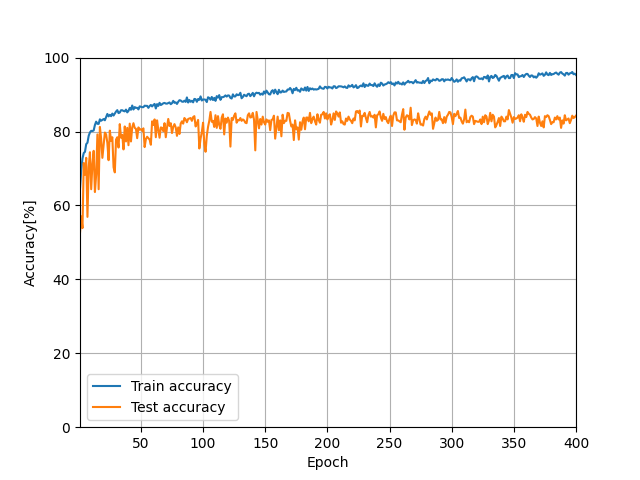
\includegraphics[keepaspectratio, scale=0.45]{./chapter4/acc_cnn.png}
    \caption{CNNでの正答率}
    \label{fig_acc_cnn}
  \end{minipage}
  \begin{minipage}[b]{0.45\linewidth}
    \centering
    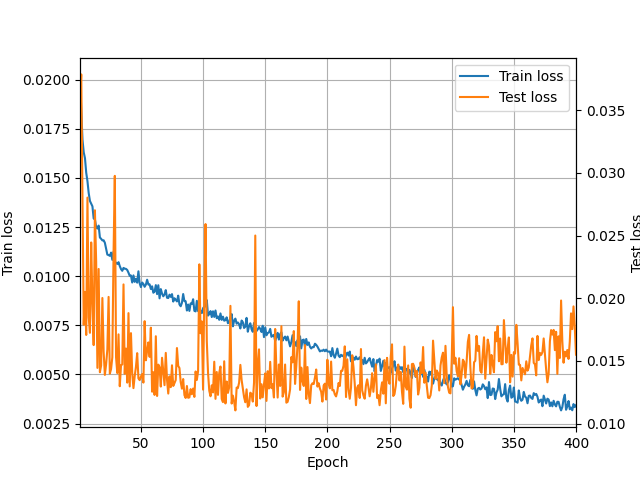
\includegraphics[keepaspectratio, scale=0.45]{./chapter4/loss_cnn.png}
    \caption{CNNでの誤差}
    \label{fig_loss_cnn}
  \end{minipage}
\end{figure}

\begin{figure}[htbp]
  \begin{minipage}[b]{0.45\linewidth}
    \centering
    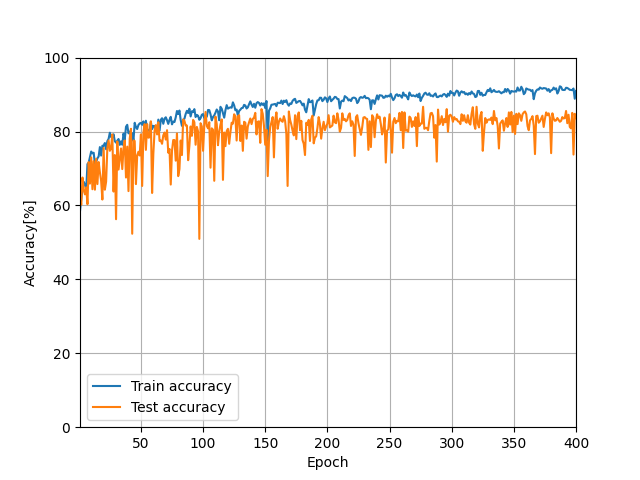
\includegraphics[keepaspectratio, scale=0.45]{./chapter4/acc_bc.png}
    \caption{BinaryConnectでの正答率}
    \label{fig_acc_bc}
  \end{minipage}
  \begin{minipage}[b]{0.45\linewidth}
    \centering
    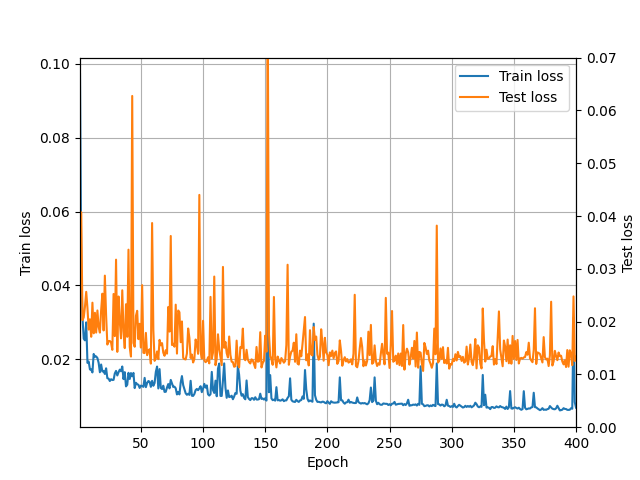
\includegraphics[keepaspectratio, scale=0.45]{./chapter4/loss_bc.png}
    \caption{BinaryConnectでの誤差}
    \label{fig_loss_bc}
  \end{minipage}
\end{figure}

\begin{figure}[htbp]
  \begin{minipage}[b]{0.45\linewidth}
    \centering
    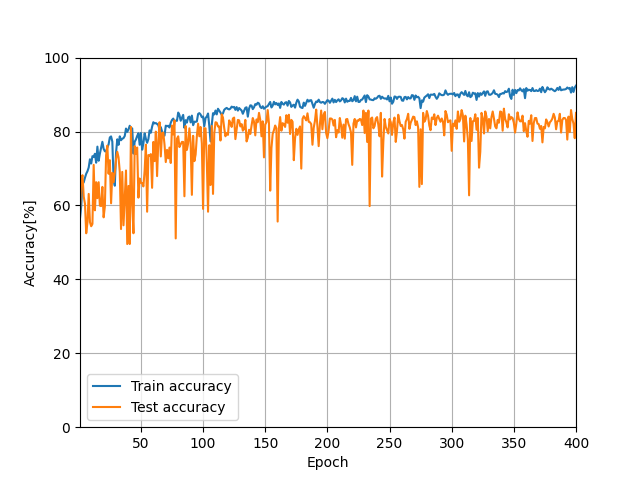
\includegraphics[keepaspectratio, scale=0.45]{./chapter4/acc_bwb.png}
    \caption{2値化したバイアスを持つBinaryConnectでの正答率}
    \label{fig_acc_bwb}
  \end{minipage}
  \begin{minipage}[b]{0.45\linewidth}
    \centering
    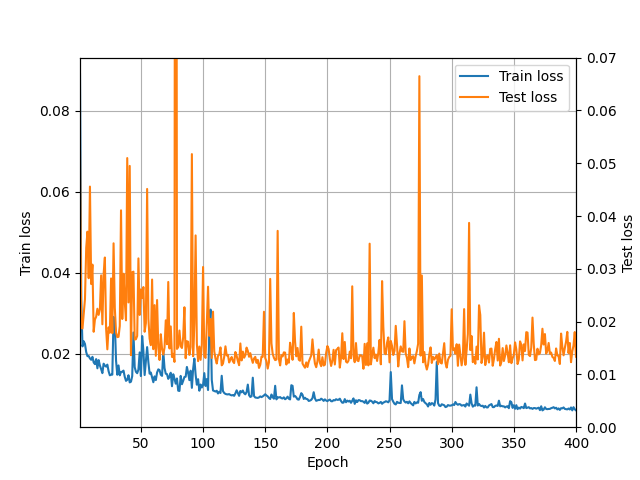
\includegraphics[keepaspectratio, scale=0.45]{./chapter4/loss_bwb.png}
    \caption{2値化したバイアスを持つBinaryConnectでの誤差}
    \label{fig_loss_bwb}
  \end{minipage}
\end{figure}

\begin{figure}[htbp]
  \begin{minipage}[b]{0.45\linewidth}
    \centering
    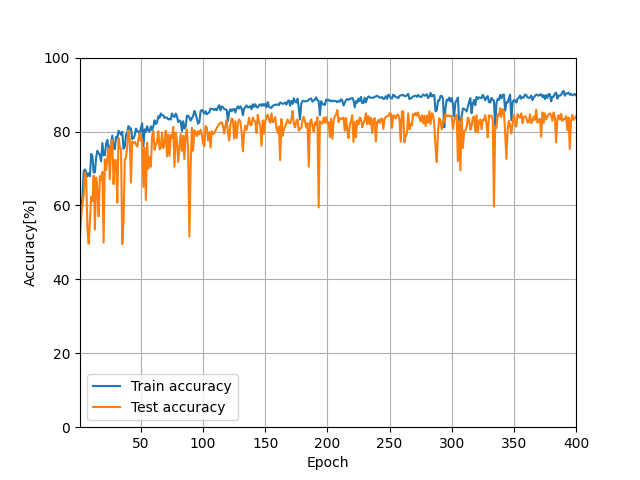
\includegraphics[keepaspectratio, scale=0.45]{./chapter4/acc_bc_nb.png}
    \caption{バイアスを消去したBinaryConnectでの正答率}
    \label{fig_acc_bc_nb}
  \end{minipage}
  \begin{minipage}[b]{0.45\linewidth}
    \centering
    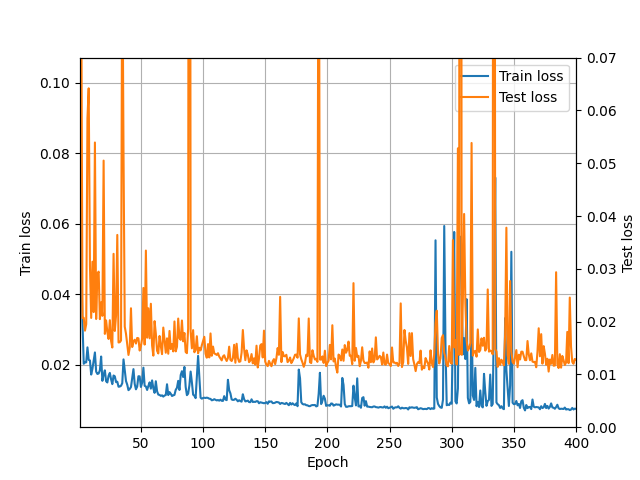
\includegraphics[keepaspectratio, scale=0.45]{./chapter4/loss_bc_nb.png}
    \caption{バイアスを消去したBinaryConnectでの誤差}
    \label{fig_loss_bc_nb}
  \end{minipage}
\end{figure}

これらの結果より,正答率やその推移はどのネットワークも同様の傾向を示していることが分かる.CNNの誤差は250Epoch近傍から上昇傾向にあるが,3つのBinaryConnectでは200Epoch近傍まで減少傾向にあり,その後は維持をしている.このことからCNNでは250Epoch以降過学習状態にあるがBinaryConnectを用いることによってオーバーフィッティングを抑えられ高Epochでの学習にも対応できるようになっていると考えられる.

CNNに比べ3つのBinaryConncetでは判定精度にばらつきがありLossの値も大きくなっていることが分かる.各ネットワークの最終10Epochの平均正答率をまとめると以下のようになった.
\begin{itemize}
  \item CNN:83.57\%
  \item BinaryConnect:82.53\%
  \item BinaryConnect(Binarize Bias):82.30\%
  \item BinaryConnect(No Bias):82.50\%
\end{itemize}

この結果から分かる通り,BinaryConnectでは正答率にばらつきがあるが,正答率に大きな差はない.今回のネットワークの構造において,1178288個の重みを使用しており,32bitの浮動小数で表されるCNNでは重みだけで約4.7MBのメモリを消費する.しかしBinaryConnectを使用することで重みは約117KBまで削減することができる.ここまでの情報量を削減して同等の正答率を確保できることは,BinaryConnectが計算リソースの削減に有効であるといえる.また,バイアスを2値化,消去しても正答率への影響は少ない.バイアスは重みほど計算リソースを圧迫しないが,32bitの浮動小数を持つ.消去しても同等の性能を示すことはこの手法も計算コストの削減として有効であるといえる.

\section{BinaryConnectの重みの推移}
BinaryConnectの正答率はEpochごとのばらつきが大きくなっている.これは0付近で揺れている重みを強制的に2値化するためフィルタが大きく変化することによるものではないかと考えた.図\ref{fig_acc_bc}の実験結果で,378Epoch目の正答率は約84.92\%,379Epoch目の正答率は83.77\%,380Epoch目の正答率は74.14\%である.378Epochと379Epochでは正答率がほぼ同じだが,379Epochと380Epochでは約10\%低下している.そこで各Epochにおける層ごとの-1の個数の変化率を検証した.その結果を表\ref{table_parameter_transition}にまとめる.
\begin{table}
  \caption{Epochごとの重みの変化率}
  \label{table_parameter_transition}
  \centering
  \begin{tabular}{ccc}
    \hline
    Layer & 378$\to$379Epoch(\%) & 379$\to$380Epoch(\%) \\
    \hline \hline
    $C_1$ & 0.833 & 2.439\\
    $C_2$ & 0.476 & 0.395\\
    $C_3$ & 1.244 & 0.256\\
    $C_4$ & 0.061 & 0.492\\
    $C_5$ & 0.030 & 0.070\\
    $C_6$ & 0.344 & 0.257\\
    $C_7$ & 0.226 & 0.002\\
    $C_8$ & 0.094 & 0.058\\
    $C_9$ & 0.013 & 0.117\\
    $C_{10}$ & 0.099 & 0.092\\
    全結合層 & 0 & 1.090\\
    \hline
  \end{tabular}
\end{table}

この結果をみると正答率が変わらないときに比べ,減少する時は入力層,出力層においての-1の変化率が大きくなっていることが分かる.隠れ層では両者に大きな差はないことから,重みの正答率への影響は入口や出口で顕著に現れると考えられる.重みのばらつきを抑え正答率を上げるためにはネットワークの入口,出口付近の重みをクリッピングしたり,計算リソースを犠牲にして重みのビット数を増やしたりなどの対策が考えられる.

\section{各ネットワークにおける不正解の傾向}